\subtop{Kreuzungsminimierung}{-1.45}
\vspace*{-0.5\baselineskip}
\begin{description}
	\item[Beobachtung:] Die Anzahl an Kreuzungen ist nicht abhängig von den genauen $x$-Koordinaten, sondern von der Permutation (Ordnung) der Knoten. Es ist einfach Ordnungen zu spezifizieren für $L_1,L_2$ durch Koordinaten-Vektoren $X_1$ und $X_2$.
\end{description}
\begin{itemize}[itemsep=-1pt]
	\item betrachtet wird ein eingeschränktes Kreuzungsminimierungsproblem
	\item ist schon $\mathcal{NP}$-schwer
	\item Zur Optimierung gibt es den Ansatz des \glqq layer-by-layer sweep\grqq (\algobreak\algo{layer-by-layer sweep}{\begin{algorithm}[H]
	\SetAlgoVlined
	\SetKwProg{Fn}{Function}{}{end}
	\KwIn{Lagen-Graph $G=(L_0\cup \dots\cup L_h,E)$}
%	\KwOut{Stack $S$ mit Knoten der konvexen Hülle $H(Q)$ im Uhrzeigersinn geordnet (von oben nach unten in $S$)}
	\BlankLine
	\begin{enumerate}
		\item wähle eine zufällige Permutation für $L_0$
		\item wiederhole für die angrenzenden Layer $L_i,L_{i+1}$:\\
			minimiere die Anzahl an Kreuzungen durch umsortieren von $L_{i+1}$ ($L_i$ bleibt fixiert)
		\item wiederhole Schritt 2 in umgekehrter Reihenfolge (von $L_h$ nach $L_0$)
		\item wiederhole Schritt 2 und 3 bis die Anzahl an Kreuzungen sich nicht mehr verringert
		\item wiederhole Schritt 1-4 mit anderer Start-Permutation
	\end{enumerate}
\end{algorithm}})
\end{itemize}
\subsection{Zwei-Lagen-Kreuzungsminimierung}
\begin{itemize}[itemsep=-1pt]
	\item Graph ist gegeben durch eine Partition von $V$ auf zwei Lagen $L_1,L_2$
	\item gesucht sind Anordnungen $X_1,X_2$ von $L_1,L_2$ sodass die Anzahl der Kantenpaare, die sich kreuzen möglichst gering ist
	\item $X_1$ sei fest, gesucht ist also nur noch die Anordnung $X_2$ von $L_1$, dass die Anzahl der Kreuzungen minimal ist
	\item für $X_1,X_2$ definieren wir
		\begin{itemize}
			\item $cross(G,X_1,X_2)=\# ((u,w),(v,z))$ mit $X_1(u)<X_1(v) \wedge X_2(w)>X_2(z)$ oder umgekehrt (Anzahl der Kreuzungen für die Ordnungen $X_1,X_2$)
			\item $opt(G,X_1)=\min\limits_{X_2}\{cross(G,X_1,X_2)\}$
			\item für $u,v\in L_1,~X_1(u)<X_1(v)$ definieren wir die \textbf{Kreuzungszahl} $c_{uv}$:
				\[c_{uv}=|\{(u,w),(v,z)\in E~:~X_2(z)<X_2(w)\}|\]
				für $u=v$ gilt $c_{uv}=0,~\forall u\in L_2$
		\end{itemize}
	\item für einen 2-Layer-Graph gilt:
		\begin{enumerate}[itemsep=-1pt]
			\item $cross(G,X_1,X_2)=\sum\limits_{\substack{u,v\in L_2\\X_2(u)<X_2(v)}} c_{uv}$
			\item $opt(G,X_1)\geq \sum\limits_{\substack{u,v\in L_2\\u\neq v}}\min\{c_{uv},c_{v,u}\}$
		\end{enumerate}
		2. gilt, da für jede Ordnung (auch die optimale) entweder $X_2(u)<X_2(v)$ oder andersherum gilt
	\item es gibt verschiedene \textit{\textbf{Heuristiken}} zur Reduktion von Kreuzungen, zum Beispiel die \textit{Greedy-switch-Heuristik} (\algo{Greedy switch Heuristik}{\begin{algorithm}[H]
	\SetAlgoVlined
	\SetKwProg{Fn}{Function}{}{end}
	\KwIn{zweichichtiger Graph (two Layer) $G=(L_1\cup L_2,E)$ mit Kreuzungszahlen $c_{uv}$}
	\BlankLine
	\Begin{
		\Repeat{
			$cross(G,X_1,X_2)$ sich nicht mehr verändert
		}{
			\For{$v=1,\dots,|L_2|-1$}{
				\If{$c_{v(v+1)}>c_{(v+1)v}$}{
					tausche die Positionen von $v$ und $v+1$
				}
			}
		}
	}
\end{algorithm}})
\end{itemize}
\begin{description}
	\item[Bemerkungen:]\ \\\vspace*{-\baselineskip}
		\begin{itemize}[itemsep=-1pt]
			\item Berechnung der Kreuzungszahlen benötigt im naiven Ansatz $\BigO(|E|^2)$, beim verbesserten $\BigO(|L_1|+|L_2|+|E|+\sum\limits_{u,v} c_{uv})$
			\item Komplexität von Greedy switch ist $\BigO(|L_2|^2)$ (jeder Scan benötigt $\BigO(|L_2|)$ Zeit; es gibt höchstens $\BigO(|L_2|)$ Scans)
			\item kein komplettes Neuberechnen von $X_2$, nur Verbesserung der aktuellen Berechnung (nicht alle Aufrufe des Algorithmus verbessern die Darstellung des Graphen)
		\end{itemize}
\end{description}
\topbreak
\vspace*{-2\baselineskip}
\subsubsection{Schwerpunkts-Zentrum-Heuristik (barycenter heuristic)}
Hier wird der Schwerpunkt eines Knotens auf $L_2$ berechnet und so die Reihenfolge der Knoten in $X_2$ festgelegt, \algo{Barycenter Heuristik}{\begin{algorithm}[H]
	\SetAlgoVlined
	\SetKwProg{Fn}{Function}{}{end}
	\KwIn{zweichichtiger Graph (two Layer) $G=(L_1\cup L_2,E)$ mit Kreuzungszahlen $c_{uv}$}
	\KwOut{$G$ mit weniger Kreuzungen, mit $0$ Kreuzungen, falls $G$ kreuzungsfrei}
	\BlankLine
	\Begin{
		\For{$v=1,\dots,|L_2|$}{
			$bary(v)=\dfrac{1}{deg(v)}\sum\limits_{u\in N(v)}X_1(u)$\\
			\If{$bary(v)=bary(w),w\neq v$}{
				trenne die Knoten durch einen kleinen Abstand
			}
		}
		sortiere $L_2$ nach den bary-Werten und setze $X_2$ entsprechend
	}
\end{algorithm}}
\begin{description}
	\item[Bemerkungen:] \ \\ \vspace*{-\baselineskip}
		\begin{itemize}[itemsep=-1pt]
			\item Komplexität: $\BigO(|L_2|+|E|+|L_2|\log|L_2|)$
			\item $\BigO(\sqrt{n})$-Annäherung: {\color{red}\textbf{TODO}}%TODO
			\item \example{\text{Schlechter Fall}}{
				\ \\ \vspace*{-\baselineskip}
				\begin{minipage}{0.5\textwidth}
					\hspace*{-1cm}\usetikzlibrary{decorations.pathreplacing}
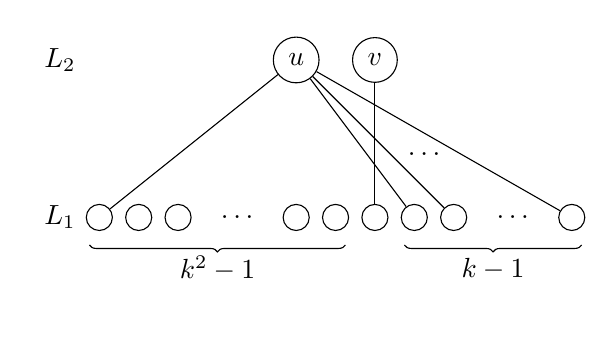
\begin{tikzpicture}[every node/.style={draw,circle},xscale=0.5]

\node(1) at (0,0) {};
\node(2) at (1,0) {};
\node(3) at (2,0) {};
\node(4) at (5,0) {};
\node(5) at (6,0) {};
\node(6) at (7,0) {};
\node(7) at (8,0) {};
\node(8) at (9,0) {};
\node(9) at (12,0) {};
\node(u) at (5,2) {$u$};
\node(v) at (7,2) {$v$};
\node[draw=none] at(3.5,0){$\ldots$};
\node[draw=none] at(10.5,0){$\ldots$};
\node[draw=none] at(8.25,0.8){$\ldots$};
\node[draw=none] at(-1,0){$L_1$};
\node[draw=none] at(-1,2){$L_2$};

\draw(1)--(u);
\draw(7)--(u);
\draw(8)--(u);
\draw(9)--(u);

\draw(6)--(v);
\draw[decorate,decoration={brace}](6.25,-0.35)to(-0.25,-0.35);
\draw[decorate,decoration={brace}](12.25,-0.35)to(7.75,-0.35);

\node[draw=none] at(3,-0.65){$k^2-1$};
\node[draw=none] at(10,-0.65){$k-1$};
\end{tikzpicture}
				\end{minipage}
				\begin{minipage}{0.35\textwidth}
					$bary(u)=k^2-\frac{k}{2}-\frac{1}{2}$\\
					$bary(v)=k^2$\\
					$\Rightarrow X_2(u)<X_2(v)$\\
					$\Rightarrow k-1$ Kreuzungen\\
					Optimal wäre aber $X_2(v)<X_2(u)\\
					\Rightarrow 1$ Kreuzung
				\end{minipage}
			}
		\end{itemize}
\end{description}

\subsubsection{Median-Heuristik}
Berechnung er Position auf $L_2$ mittels des Medians (\algo{Median-Heuristik}{\begin{algorithm}[H]
	\SetAlgoVlined
	\SetKwProg{Fn}{Function}{}{end}
	\KwIn{zweichichtiger Graph (two Layer) $G=(L_1\cup L_2,E)$ mit Kreuzungszahlen $c_{uv}$}
	\KwOut{$G$ mit weniger Kreuzungen, mit $0$ Kreuzungen, falls $G$ kreuzungsfrei}
	\BlankLine
	\Begin{
		\For{$v=1,\dots,|L_2|$}{
			$v_1,\dots,v_k \leftarrow N(v)$ mit $X_1(v_1)<\dots<X_1(v_k)$\\
			$m(v)\leftarrow\left\{ 
				\begin{array}{ll}
					0&N(v)=\emptyset\\
					X_1(v_{\lceil \frac{k}{2}\rceil})&\text{sonst}
				\end{array}
			\right.$\\
			\If{$m(v)_m(w), v\neq w$}{
				trenne $m(v)$ und $m(w)$ durch einen kleinen Abstand
			}
		}
		sortiere $L_2$ nach den $m$-Werten und setze $X_2$ entsprechend
		
	}
\end{algorithm}})
\begin{description}
	\item[Bemerkungen:]\ \\ \vspace*{-\baselineskip}
		\begin{itemize}
			\item Komplexität: gleich wie bei \textit{barycenter Heuristik}
			\item 3-Annäherung:{\color{red}\textbf{TODO}}%TODO
			\item \example{\text{Schlechter Fall}}{
				\ \\ \vspace*{-\baselineskip}
				\begin{minipage}{0.5\textwidth}
					\hspace*{-1cm}\usetikzlibrary{decorations.pathreplacing,arrows}
\begin{tikzpicture}[every node/.style={draw,circle},xscale=0.5]

\node(1) at (0,0) {};
\node(2) at (1,0) {};
\node(3) at (2,0) {};
\node(4) at (3,0) {};
\node(5) at (4,0) {};
\node(6) at (5,0) {};
\node(7) at (6,0) {};
\node(8) at (8,0) {};
\node(9) at (9,0) {};
\node(10) at (10,0) {};
\node(11) at (11,0) {};
\node(12) at (12,0) {};
\node(13) at (13,0) {};
\node(14) at (14,0) {};
\node(u) at (6,2) {$u$};
\node(v) at (8,2) {$v$};

\node[draw=none] at(-1,0){$L_1$};
\node[draw=none] at(-1,2){$L_2$};

\foreach \x in {4,5,6,7,12,13,14}
	\draw(u)to(\x);
\foreach \x in {1,2,3,8,9,10,11}
	\draw(v)to(\x);

\draw[decorate,decoration={brace}](2.25,-0.35)to(-0.25,-0.35);
\draw[decorate,decoration={brace}](6.25,-0.35)to(2.75,-0.35);
\draw[decorate,decoration={brace}](11.25,-0.35)to(7.75,-0.35);
\draw[decorate,decoration={brace}](14.25,-0.35)to(11.75,-0.35);

\node[draw=none] at(1,-0.65){$k$};
\node[draw=none] at(13,-0.65){$k$};
\node[draw=none] at(4.5,-0.65){$k+1$};
\node[draw=none] at(9.5,-0.65){$k+1$};

\node[draw=none,rectangle] (mu) at (6,-1.5) {$med(u)$};
\node[draw=none,rectangle] (mv) at (8,-1.5) {$med(v)$};

\draw[->,>=triangle 60](mu)--(6,-0.5);
\draw[->,>=triangle 60](mv)--(8,-0.5);
\end{tikzpicture}
				\end{minipage}
				\begin{minipage}{0.35\textwidth}
					$k(k+1)+k^2+k(k+1)$ Kreuzungen\\
					Optimal wäre aber $X_2(v)<X_2(u)\\
					\Rightarrow (k+1)^2$ Kreuzungen
				\end{minipage}
			}
		\end{itemize}
\end{description}
\subsection{Allgemeine Bemerkungen}
\begin{itemize}[itemsep=-1pt]
	\item optimale Lösung kann mit Hilfe von \textit{Integer Linear Programmin} berechnet werden, aber es kann keine polynomielle Zeit gewährleistet werden
	\item in der Praxis gibt es keinen klaren Sieger (der Heuristiken)\\
		$\Rightarrow$ am häufigsten wird die \textit{hybrid}-Methode verwendet:
			\begin{enumerate}
				\item Median
				\item Bindungen brechen mit der barycenter Heuristik
				\item verbessern mit Greedy switch
			\end{enumerate}
\end{itemize}